\documentclass[../readings.tex]{subfiles}

\begin{document}
\subsection{Overdetermined Systems and Least Squares}
\label{subsec:least-squares}

\textBox{%
So far, we have focused on solving square systems of linear equations $\bA\bx = \bb$ where $\bA \in \mathbb{R}^{n \times n}$. In many real-world applications, however, we encounter overdetermined systems where we have more equations than unknowns, leading to systems that typically have no exact solution. The method of least squares provides a powerful approach to finding the "best" approximate solution to such systems.
}

\subsubsection{Overdetermined Systems}
\addDef{Overdetermined Systems and Least Squares}{%
An overdetermined linear system has the form 
$$
\bA \bx = \bb,
$$
where $\bA \in \mathbb{R}^{m \times n}$ with $m > n$ and $\bb \in \mathbb{R}^m$. Since $\bA$ maps from $\mathbb{R}^n$ to $\mathbb{R}^m$, its range is at most $n$-dimensional. When $m > n$ and $\bb$ is a general vector in $\mathbb{R}^m$, it typically lies outside the range of $\bA$, meaning no exact solution exists.}

\subsubsection{Least Squares}
\addDef{Least Squares}{
The \textbf{least squares problem} addresses this by finding the vector $\hat{\bx}$ that minimizes the sum of squared residuals:
$$
\hat{\bx} = \argmin_{\bx \in \mathbb{R}^n} \| \bA \bx - \bb \|_2^2
$$

This formulation seeks the $\bx$ that makes $\bA\bx$ as close as possible to $\bb$ in the Euclidean norm sense.
}

\addNote{%
Overdetermined systems arise naturally in data fitting, statistical regression, signal processing, and many scientific applications where we have more measurements (equations) than parameters (unknowns). For example, when fitting a line to a set of data points, we typically have many more points than the two parameters needed to define a line.
}

\textBox{%
Geometrically, the least squares solution represents the orthogonal projection of $\bb$ onto the column space of $\bA$. When $\bA\hat{\bx}$ is this projection, the residual vector $\br = \bb - \bA\hat{\bx}$ is orthogonal to the column space, making it the shortest possible residual vector.

\begin{figure}[!htbp]
\centering
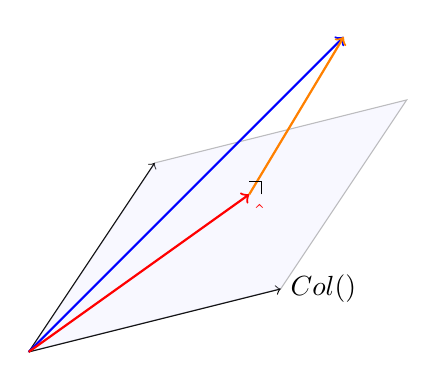
\begin{tikzpicture}[scale=0.8]
    % Column space
    \draw[->] (0,0) -- (4,1) node[right] {$\text{Col}(\bA)$};
    \draw[->] (0,0) -- (2,3) node[above] {};
    \draw[fill=blue!10, nearly transparent] (0,0) -- (4,1) -- (6,4) -- (2,3) -- cycle;
    
    % Vector b
    \draw[->, thick, blue] (0,0) -- (5,5) node[right] {$\bb$};
    
    % Projection
    \draw[->, thick, red] (0,0) -- (3.5,2.5) node[below right] {$\bA\hat{\bx}$};
    
    % Residual
    \draw[->, thick, orange] (3.5,2.5) -- (5,5) node[midway, above left] {$\br$};
    
    % Orthogonality marker
    \draw (3.7,2.5) -- (3.7,2.7) -- (3.5,2.7);
\end{tikzpicture}
\end{figure}
}

\addDef{Deriving the Normal Equations}{%
To find the minimizer of $f(\bx) = \|\bA \bx - \bb\|_2^2$, we can expand this expression:
$$
f(\bx) = (\bA \bx - \bb)^T (\bA \bx - \bb) = \bx^T \bA^T \bA \bx - 2 \bb^T \bA \bx + \bb^T \bb
$$

Since $\bb^T \bb$ is constant with respect to $\bx$, we can focus on minimizing:
$$
g(\bx) = \bx^T \bA^T \bA \bx - 2 \bb^T \bA \bx
$$

Setting the gradient to zero (a necessary condition for a minimum):
$$
\nabla_{\bx} g(\bx) = 2 \bA^T \bA \bx - 2 \bA^T \bb = \mathbf{0}
$$

This leads to the \textbf{normal equations}:
$$
\bA^T \bA \bx = \bA^T \bb
$$

When $\bA$ has full column rank (i.e., its columns are linearly independent), $\bA^T \bA$ is invertible, and the unique least squares solution is:
$$
\hat{\bx} = (\bA^T \bA)^{-1} \bA^T \bb
$$
}

\addNote{%
The term "normal equations" comes from the fact that the residual $\br = \bb - \bA\hat{\bx}$ is normal (perpendicular) to the column space of $\bA$. This orthogonality principle is fundamental to least squares theory and follows directly from the normal equations:
$$
\bA^T (\bb - \bA\hat{\bx}) = \mathbf{0}
$$
This equation confirms that each column of $\bA$ is orthogonal to the residual vector.
}

\addExmpl{
Consider fitting a straight line $y = mx + b$ to the data points $(1,2)$, $(2,3)$, $(3,5)$, and $(4,4)$. 

We can rewrite the line equation in matrix form:
$$
\begin{pmatrix} 1 & 1 \\ 1 & 2 \\ 1 & 3 \\ 1 & 4 \end{pmatrix}
\begin{pmatrix} b \\ m \end{pmatrix} =
\begin{pmatrix} 2 \\ 3 \\ 5 \\ 4 \end{pmatrix}
$$

This is an overdetermined system with $\bA \in \mathbb{R}^{4 \times 2}$ and $\bb \in \mathbb{R}^4$. Computing the normal equations:
$$
\bA^T\bA = \begin{pmatrix} 1 & 1 & 1 & 1 \\ 1 & 2 & 3 & 4 \end{pmatrix}
\begin{pmatrix} 1 & 1 \\ 1 & 2 \\ 1 & 3 \\ 1 & 4 \end{pmatrix} =
\begin{pmatrix} 4 & 10 \\ 10 & 30 \end{pmatrix}
$$

$$
\bA^T\bb = \begin{pmatrix} 1 & 1 & 1 & 1 \\ 1 & 2 & 3 & 4 \end{pmatrix}
\begin{pmatrix} 2 \\ 3 \\ 5 \\ 4 \end{pmatrix} =
\begin{pmatrix} 14 \\ 41 \end{pmatrix}
$$

Solving $(\bA^T\bA)\hat{\bx} = \bA^T\bb$:
$$
\begin{pmatrix} 4 & 10 \\ 10 & 30 \end{pmatrix}
\begin{pmatrix} b \\ m \end{pmatrix} =
\begin{pmatrix} 14 \\ 41 \end{pmatrix}
$$

We get $\hat{b} = 1.3$ and $\hat{m} = 0.9$, giving the best-fit line $y = 0.9x + 1.3$.
}

\subsubsection{QR Based Least Squares}
\addDef{QR Based Least Squares}{%
While the normal equations provide a direct formula, they can lead to numerical instability, especially when $\bA$ is ill-conditioned. This is because forming $\bA^T\bA$ effectively squares the condition number:
$$
\kappa(\bA^T\bA) = \kappa(\bA)^2
$$
To address this, we can use the $QR$ decomposition. When $\bA = \bQ\bR$ where $\bQ$ has orthonormal columns and $\bR$ is upper triangular, the least squares problem becomes:
$$
\min_{\bx} \|\bQ\bR \bx - \bb\|_2 = \min_{\bx} \|\bR \bx - \bQ^T \bb\|_2
$$
The solution is found by solving the triangular system:
$$
\bR \bx = \bQ^T \bb
$$
}

\textBox{%
The QR and SVD approaches avoid forming $\bA^T\bA$ explicitly, thus preserving numerical precision. For large, sparse systems, iterative methods like Conjugate Gradient applied to the normal equations (CGNE) can be more efficient than direct factorization methods.
}

\addExmpl{%
Continuing with our line-fitting example, we can use the QR decomposition of $\bA$ to solve the least squares problem.

If $\bA = \bQ\bR$ where:
$$
\bQ \approx \begin{pmatrix} 
0.5 & -0.67 & ... \\ 
0.5 & -0.22 & ... \\ 
0.5 & 0.22 & ... \\ 
0.5 & 0.67 & ... 
\end{pmatrix}
\quad \text{and} \quad
\bR \approx \begin{pmatrix} 
2 & 5 \\ 
0 & 3.74 \\ 
0 & 0 \\
0 & 0
\end{pmatrix}
$$

Then the solution can be found by solving:
$$
\begin{pmatrix} 
2 & 5 \\ 
0 & 3.74
\end{pmatrix}
\begin{pmatrix} b \\ m \end{pmatrix} =
\begin{pmatrix} 7 \\ 3.37 \end{pmatrix}
$$

where the right-hand side is $\bQ^T\bb$. This triangular system is easily solved by back-substitution, yielding the same solution as before but with better numerical stability.
}

\addNote{%
The least squares method can be extended in many ways (covered in introductory machine learning courses), including:
\begin{itemize}
    \item Weighted least squares, where some measurements are given more importance than others
    \item Regularized least squares (e.g., ridge regression, LASSO), which address ill-conditioning and prevent overfitting
    \item Nonlinear least squares for fitting more complex models
\end{itemize}
These extensions maintain the core principle of minimizing the sum of squared residuals while incorporating additional constraints or structures.
}

\end{document}